\documentclass[10pt,a4paper]{article}

\usepackage[utf8]{inputenc}
\usepackage[margin=1.2in]{geometry}
\usepackage[french]{babel}
\usepackage{amsmath}
\usepackage{amsfonts}
\usepackage{graphicx}
\usepackage{hyperref}
\usepackage[nottoc, notlof, notlot]{tocbibind}
\hypersetup{colorlinks=true,citecolor=black,filecolor=black,linkcolor=black,urlcolor=black}
\setlength{\parindent}{0.6cm} 
\setlength{\parskip}{0.10cm}
\usepackage[automark]{scrpage2}
\usepackage{color, colortbl}
\usepackage[table]{xcolor}


\ihead[]{Equipe Navigation}
\ohead[]{Plan Qualité}



\begin{document}
\pagestyle{scrheadings}

\begin{titlepage}


\newcommand{\HRule}{\rule{\linewidth}{0.5mm}} 

\center

\textsc{\Large Université Paul Sabatier}\\[1cm] 

\includegraphics[scale=0.3]{UPS.jpg}\\[0.6cm] 


\textsc{Master Intelligence Artificielle et \\ 
Reconnaissance des Formes \\ Master Robotique : Décision et Commande}\\[3cm] 

\HRule \\[0.4cm]
{ \huge \bfseries Plan de Développement Qualité}\\[0.4cm] 
\LARGE Navigation Autonome de Robot Mobile

\HRule \\[1.5cm]
 

\begin{minipage}{0.4\textwidth}
\begin{flushleft} \large
\emph{Auteur:}\\
\href{mailto:thibaut.aghnatios@laposte.net}{Thibaut \textsc{Aghnatios} }  \\
\href{mailto:bouchetmarinee@gmail.com}{Marine \textsc{Bouchet} } \\
\href{mailto:bruno.dato.meneses@gmail.com}{Bruno \textsc{Dato} } \\
\href{mailto:klempka.tristan@gmail.com}{Tristan \textsc{Klempla} } \\
\href{mailto:lagoute.31@gmail.com}{Thibault \textsc{Lagoute} }  
\end{flushleft}
\end{minipage}
~
\begin{minipage}{0.4\textwidth}
\begin{flushright} \large
\emph{Tuteur:} \\
\href{mailto:lerasle@laas.fr}{Frédéric \textsc{Lerasle}}\\
\href{mailto:michael.lauer@laas.fr}{Michaël \textsc{Lauer}} \\
\href{mailto:taix@laas.f}{Michel \textsc{Taix}}
\end{flushright}
\end{minipage}\\[1cm]

%\large 29 août 2016}\\[1.1cm] 
%\includegraphics[scale=0.3]{logo.jpeg} 
% laaaaaaaaaaaaaaaaaaaaaaaaaaaaaaaaaaaaaaaaaaaaaaaaaas
 

\end{titlepage}

\newpage


\subsection*{Suivi du document}

\begin{center}
    \begin{tabular}{| l | l | l | l | l |}
    \hline
     \rowcolor{gray} Nom du document & Version Majeure & Version Majeure & Date de création & Dernière version \\ \hline
    PDDQ & A & 0 & 27/10/2016 & 07/11/2016 \\ \hline
    \end{tabular}
\end{center}


\subsection*{Auteurs du document}

\begin{center}
    \begin{tabular}{| l | l | l | l |}
    \hline
    \rowcolor{gray} Rédaction & Intégration & Relecture & Validation Interne \\ \hline
    Equipe & Marine Bouchet & Bruno Dato, Thibaut Aghnatios & 07/11/2016 \\ \hline
    \end{tabular}
\end{center}

\subsection*{Validation du document}

\begin{center}
    \begin{tabular}{| l | l | l | l |}
    \hline
     \rowcolor{gray} Validation & Nom & Date & Visa \\ \hline
    & & & \\
     \hline
    \end{tabular}
\end{center}

\subsection*{Liste de diffusion}

Le plan qualité de projet est diffusé à l’ensemble .... 

\subsection*{Historiques de révision}

\begin{center}
    \begin{tabular}{| l | l | l | l |}
    \hline
     \rowcolor{gray} Version & Modification apportée & Auteur & Date \\ \hline
    & & & \\
     \hline
    \end{tabular}
\end{center}

\newpage
\tableofcontents
\newpage
	

\section{[AMODIFIER] Introduction}
\label{sec:introduction}

La structure et le contenu de ce Plan Qualité de Projet ont été élaborés dans le cadre du projet « Navigation autonome de robots mobiles » proposé aux étudiants de deuxième année du Master  Intelligence Artificielle et Reconnaissance des Formes » de l'Université Paul Sabatier à Toulouse.

Il a pour objectif la définition et la description des différentes dispositions à mettre en œuvre pour un développement optimal du projet afin d’en assurer la qualité et d’atteindre les résultats attendus. Plus précisément, sont déterminés, d’un commun accord :
\begin{itemize}
\item l’organisation globale du projet 
\item le plan de gestion et de développement du projet
\item les droits et les devoirs de chaque partie prenante
\item la répartition des responsabilités entre les organismes dans la structure
\item les plans de développement et de gestion du projet
\item les outils qui seront adoptés 
\end{itemize}

Après acceptation par le client, ce plan deviendra le document contractuel applicable en matière de gestion et d’assurance qualité entre le Titulaire et le Client durant la durée totale du projet. La responsable qualité s’assurera qu’il est effectivement appliqué. Il ne pourra subir aucune modification sans accord préalable du Client. En cas de divergence entre les exigences et le plan qualité, les exigences s’appliqueront en priorité.

% -------------------------------

\section{Présentation du projet}
\label{sec:presentation}

\subsection{[OK] Contexte}

\subsubsection{Master IARF et RODECO}

Le master « Intelligence Artificielle et Reconnaissance des Formes » (IARF) a comme objectif de former des professionnels de haut niveau capables de concevoir des solutions à des problèmes complexes utilisant des méthodes avancées de représentation et de traitement de l’information, faisant appel à des techniques d’intelligence artificielle (IA) et de reconnaissance des formes (RF) et d’apprentissage automatique, appliqués notamment au traitement d’images et à la robotique. 

Le master « Robotique : décision et commande » (RODECO) a pour vocation de \_ des connaissances dans le domaine de l’automatique par des enseignements avancés autour de la robotique, de l’informatique et de la commande des systèmes. Ces compétences permettent d’aborder des problématiques très actuelles comme la robotique industrielle haute performance où les aspects commande sont fondamentaux et la robotique  de service où la décision et la perception tiennent une place essentielle. Suivant ce raisonnement, deux blocs de spécialisation sont proposés en M2 : 

\begin{description}
\item [Robotique et décision] qui propose un renforcement des aspects « informatique » (intelligence artificielle, reconnaissance des formes, dialogue homme/machine), vision par ordinateur et robotique  mobile. Cette spécialisation donne les compétences nécessaires pour appréhender le domaine de la robotique de service ;
\item [Robotique et commande] qui se focalise sur le développement et l’implantation de commandes avancées pour la robotique. Cette spécialisation donne donc les compétences nécessaires pour élaborer des solutions évoluées de contrôle/commande pour la réalisation de tâches robotique haute performance.
\end{description}

Au cours de cette deuxième année, les étudiants acquièrent une double compétence en Automatique et Informatique et les capacités requises pour modéliser, analyser, concevoir et réaliser des systèmes automatiques complexes, autonomes et/ou embarqués où sont impliqués la perception (capteurs), l’analyse (traitement de signal, audio, image, vidéo), le raisonnement et la décision (incertitude, reconnaissance de formes, contraintes) et de l’action (commande, robotique).
  
\subsubsection{Contexte du projet}

Le projet de Master 2 permet de mettre en commun et en pratique les connaissances acquises dans ces trois parcours dans un but commun. En l’occurrence, sur le projet « Navigation autonome de robots mobiles », Tristan et Marine font parti du parcours IARF, Thibaut et Bruno sont issus de la spécialité Décision de RODECO et enfin, Thibault, de la spécialité Commande. 

Il se déroule tout le long de l'année, en alternance avec les blocs de cours B par tranche, nommés W, de 3, 4 et 4 semaines.

\newcolumntype{g}{>{\columncolor{gray}}c}
\begin{table}[ht]
\centering
\begin{tabular}{g|c|g|c|g|c}
\hline
 B1 & W1 & B2 & W2 & B3 & W3 \\ 
\hline
 5 sem. & 3 sem. & 5 sem. & 4 sem. & 5 sem. & 4 sem. \\ 
 & 17/10 - 14/11 &  & 02/01 - 27/01 &  & 01/03 - ??/03 \\ 
\hline
\end{tabular}
\end{table}

\subsubsection{Entrées}
\begin{itemize}
\renewcommand{\labelitemi}{\mbox{\ooalign{$\checkmark$\cr\hidewidth$\square$\hidewidth\cr}}}
\item Cahier des charges
\item Documentations
\end{itemize} 

\subsubsection{Sorties}
L'objectif du projet est de répondre à un cahier des charges divisé en 4 étapes incrémentales. Le projet étant enmené à être réutilisé par la suite pour d'autres étudiants, la qualité du produit est primordiale.

\begin{itemize}
\renewcommand{\labelitemi}{$\square$}
\item Un code propre, fonctionnel et surtout facilement réutilisable 
\item Documentations
\item Robot opérationnel qui ...
\item Manuel Utilisateur
\end{itemize} 

\subsubsection{Limites}
\begin{itemize}
\item Incrémentation des solutions : difficulté d'anticiper les solutions et problèmes des étapes suivantes
\item Cours de vision 2D et de navigations en B2 et vision 3D en B3
\end{itemize} 

\subsection{[OK] Parties-prenantes}

\subsubsection{MOE} 
\begin{minipage}[t]{0.30 \textwidth} 
Thibaut \textsc{Aghnatios} \\
\href{mailto:thibaut.aghnatios@laposte.net}{thibaut.aghnatios@laposte.net} \\
Spécialité Décision \\[0.3cm]
Marine \textsc{Bouchet} \\
\href{mailto:bouchetmarinee@gmail.com}{bouchetmarinee@gmail.com} \\
Spécialité IARF \\[0.3cm]
Bruno \textsc{Dato} \\
\href{mailto:bruno.dato.meneses@gmail.com}{bruno.dato.meneses@gmail.com} \\
Spécialité Décision
\end{minipage} 
\hfill
\begin{minipage}[t]{0.46\textwidth} 
Tristan \textsc{Klempka} \\
\href{mailto:klempka.tristan@gmail.com}{klempka.tristan@gmail.com} \\
Spécialité IARF \\[0.3cm]
Thibault \textsc{Lagoute} \\
\href{mailto:lagoute.31@gmail.com}{lagoute.31@gmail.com}   \\
Spécialité Commande
\end{minipage} 

\subsubsection{MOA}
\begin{minipage}[t]{0.46 \textwidth} 
Frédéric \textsc{Lerasle} \\
\href{mailto:lerasle@laas.fr}{lerasle@laas.fr} \\
Equipe RAP, LAAS - CNRS \\[0.3cm]
Michel \textsc{Lauer} \\
\href{mailto:michael.lauer@laas.fr}{michael.lauer@laas.fr} \\
Equipe TSF, LAAS - CNRS
\end{minipage} 
\hfill
\begin{minipage}[t]{0.46\textwidth} 
Michel \textsc{Taix} \\
\href{mailto:taix@laas.fr}{taix@laas.fr} \\
Equipe GEPETO, LAAS - CNRS
\end{minipage} 

\subsubsection{Intervenants externes}
\begin{minipage}[t]{0.46 \textwidth} 
Julien \textsc{Vanderstraeten} \\
\href{mailto:julien.vanderstraeten.ups@gmail.com
}{julien.vanderstraeten.ups@gmail.com} \\
Coach
\end{minipage} 
\hfill
\begin{minipage}[t]{0.46\textwidth} 
Cyril \textsc{Briand} \\
\href{mailto:briand@laas.fr}{briand@laas.fr} \\
Coach
\end{minipage} 

\subsection{[ACOMPLETER] Contraintes}
\noindent La réalisation du projet est régie par certaines contraintes citées ci-dessous : 
\begin{itemize}
\item Robot TurtleBot
\item Planning du Master et ses jalons 
\item Connaissance partielle .... + entre les membres

\end{itemize} 

% -------------------------------



\section{Organisation du projet}
\label{sec:organisation}

\subsection{[OK] Cycle de développement}

Le développement du projet se fera selon Scrum, une méthode Agile dédiée à la gestion de projet. Cette méthode, basée sur les stratégies itératives et incrémentales, permettra de produire, à la fin de chaque « sprint », un résultat achevé et validé, pour avoir une version fonctionnelle à tout moment. Cette démarche correspond bien au cahier des charges où les étapes sont à la fois itératives et incrémentales.

Pour chaque sprint, la période initiale permettra de faire le point sur les éléments techniques du départ du projet et d'établir une liste des points à préciser ou à compléter, à savoir les charges de travail et le calendrier associé. Une nouvelle version du Plan de Qualité et du Plan de Développement adaptée à l'étape en cours sera donc produite. Chaque sprint donne lieu à une phase de codage et une phase de tests.

Scrum se différencie des autres méthodes de développement par ses avantages qui font de ce procédé une réponse à certains problèmes fréquemment rencontrés dans le développement logiciel. Pour éviter l’effet tunnel, la communication restera permanente entre les membres de l’équipe mais aussi entre l’équipe et le client, permettant une meilleure coopération à l’intérieur de l’équipe Scrum. 

SCHEMA A FAIRE !!!

\subsection{[AMODIFIER] Sprints}

\noindent Le projet est divisé en 4 étapes définies par le client : 

\begin{description}

\item [Etape 1] Réaliser une tâche robotique permettant au robot d’atteindre une balle de couleur (détecter une balle de couleur, localisation dans le repère courant du robot, aller à la balle).

\item [Etape 2] Réaliser une tâche de navigation dans un environnement supposé connu et sans obstacles pour atteindre un amer final en se déplaçant d’amer en amer (QR code : amer 2D) afin de ne pas se perdre et en optimisant un critère (distance, temps, commande,....).

\item [Etape 3] Réaliser une tâche de navigation dans un environnement supposé connu et sans obstacles inconnus pour atteindre un amer final en se déplaçant d’amer en amer (3D) afin de ne pas se perdre et en optimisant un critère (distance, temps, commande,....).

\item [Etape 4] Réaliser une tâche de balayage grâce à une modélisation par carte laser.

\end{description}

A la fin et entre chaque étape, une étude des limites et des problématiques de la prochaine étape est demandée.

\begin{figure}
  \centering
\noindent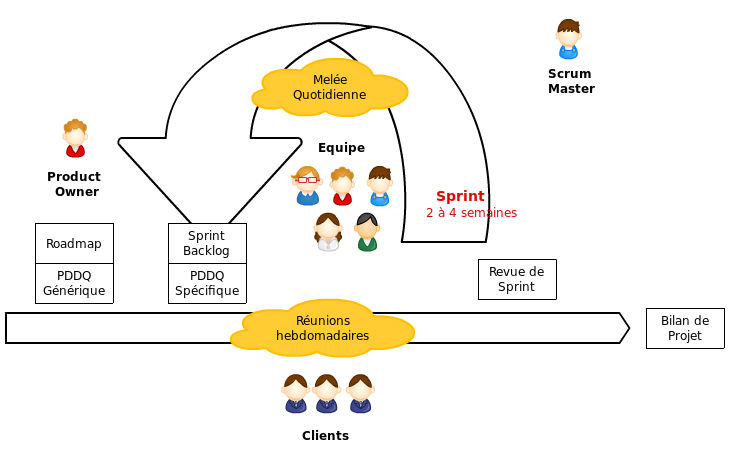
\includegraphics[width=\textwidth]{scrum.png} 
  \caption{Schéma Méthode Scrum}
\end{figure}

\section{[OK] Arbre produit}

Un arbre produit, ou \textit{Product Breakdown Structure} donne une liste exhaustive des différents livrables du projet, de manière hiérarchisée. Il permet d’avoir une vue claire des différentes fonctionnalités à développer, de décrire l’architecture logicielle et matérielle du produit à livrer, et d’en prévoir les coûts. Dans le cadre de notre projet de navigation, l’aspect budgétaire ne sera pas abordé puisqu’il s’agit d’un projet dans le cadre de la formation.
La figure suivante présente l’arbre produit du projet de navigation. Les parties encadrées correspondent aux nœuds de l’arbre, c’est à dire les groupes de fonctions à développer, tandis que les parties non encadrées correspondent aux feuilles, autrement dit aux fonctions elles-mêmes.
L’arbre produit de notre projet de navigation est décomposé en cinq parties :

\begin{description}
\item [Simulateur ROS] : concerne les différents éléments à utiliser sous ce simulateur, à savoir la modélisation de l’environnement, les différents obstacles, le calcul des trajectoires de notre robot et l’intégration des blocs au cours des différentes étapes.
\item  [Perception] : décrit l’ensemble des fonctionnalités permettant l’identification à partir d’une image. On distingue ainsi 2 groupes : la perception de l’environnement et la détection des obstacles. La détection des obstacles tient compte des différentes méthodes utilisées au cours de ce projet : le nuage de points, l’étude laser, les différentes méthodes de segmentation, etc…
\item [Localisation] : décrit les fonctions nécessaires à la navigation autonome du robot. Il devra permettre au robot de calculer sa position et déterminer son orientation grâce à des repères.
\item [Décision] : décrit les fonctions nécessaires aux différentes décisions que le robot doit prendre comme pour la génération de la trajectoire (en choisissant la trajectoire la plus courte et la plus rapide à prendre selon l’orientation du robot) et les décisions pour les différents évènements possibles.
\item [Action] : Concerne toutes les fonctions correspondant au domaine de la commande robotisée permettant le respect des consignes (atteindre une balle de couleur, un amer, …), la réalisation des mouvements, et les contraintes cinématiques. On parlera aussi de l’odométrie.
\end{description}

\begin{figure}
  \centering
\noindent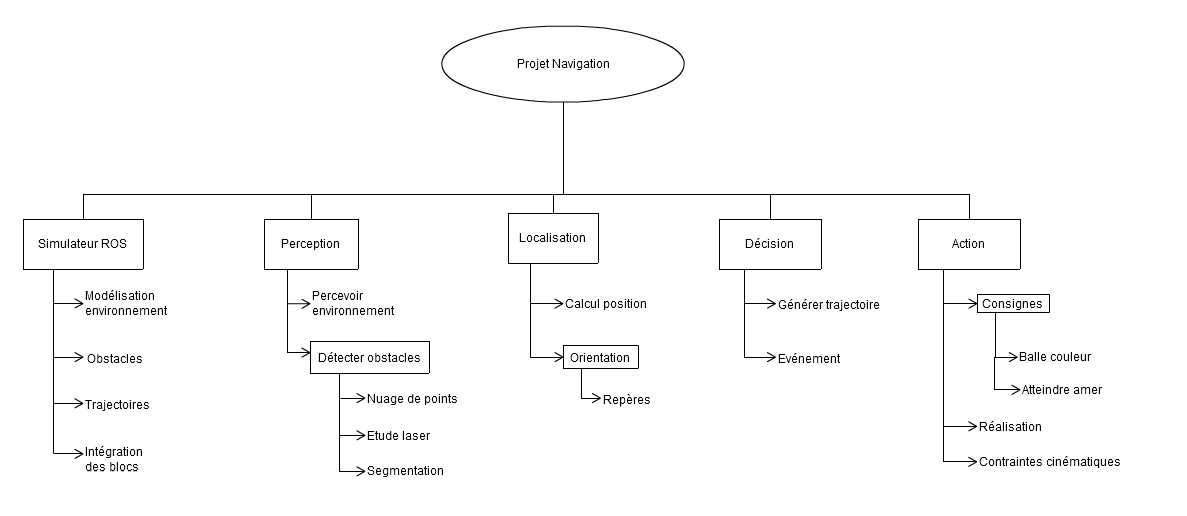
\includegraphics[width=\textwidth]{arbreproduit.png} 
  \caption{Arbre Produit}
\end{figure}

\section{[AFAIRE] RoadMap}

\section{Planning}
\label{sec:planning}

\subsection{[OK] Lôt de tâches}

Un lot de tâches, ou \textit{Work Breakdown Structure}, est une décomposition hiérarchique des tâches à effectuer dans un projet. Il permet à la fois d'avoir une représentation visuelle du travail restant à réaliser, mais aussi d'évaluer rapidement l'avancement de chacune des tâches.

La figure suivante représente nos lots de tâches pour l'ensemble du projet, nous en avons identifié six.

\begin{figure}
  \centering
\noindent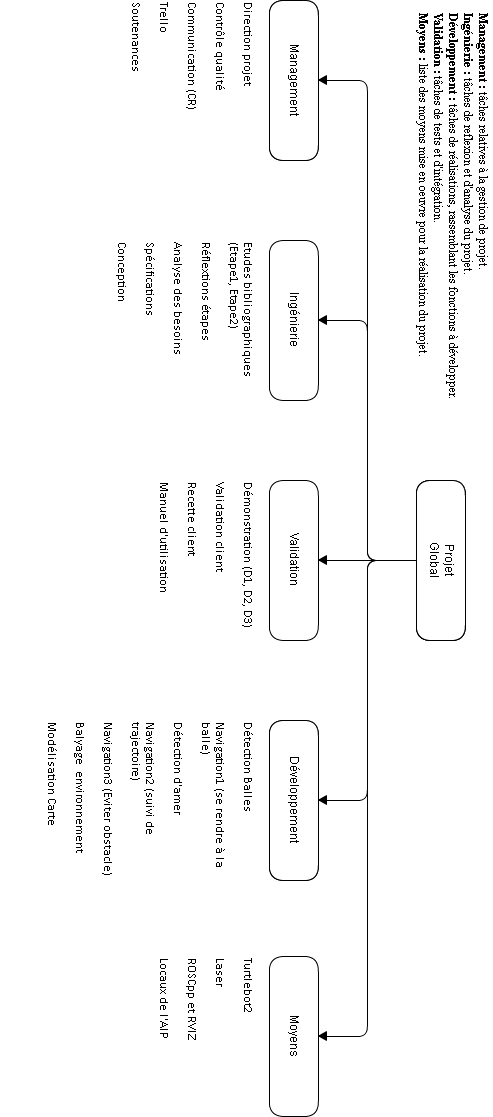
\includegraphics[width=\textwidth]{lottaches.png} 
  \caption{Lot de tâches}
\end{figure}

\subsection{[OK] Planning général}

\begin{figure}
  \centering
\noindent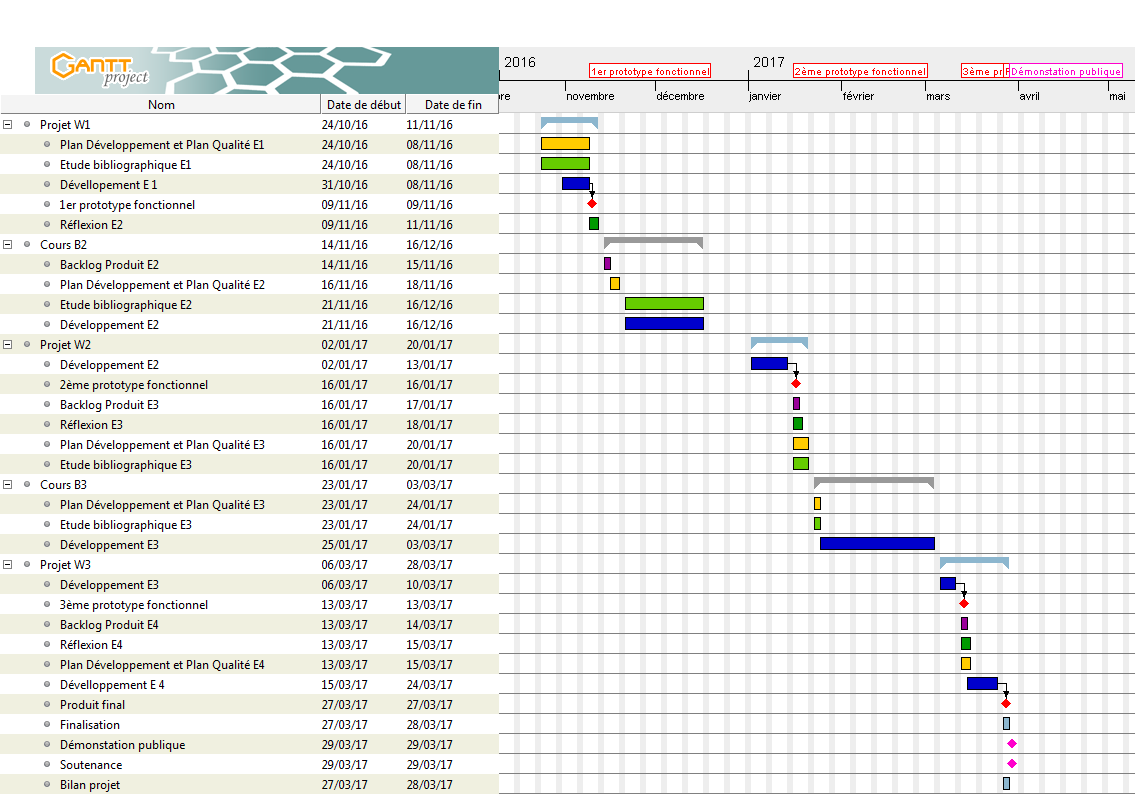
\includegraphics[width=\textwidth]{general.png} 
  \caption{Gantt du projet}
\end{figure}

\subsection{[ACONFIRMER] Livrables}

\subsubsection{Pour le client}

\begin{description}

\item [W1] du 17/10 au 14/11 : 
\begin{itemize}
\item Plan de Développement et de Qualité V1 : 8/11
\item Code de l'étape 1 et Manuel Utilisateur correspondant : 8/11
\end{itemize}

\item [W2] du 02/01 au 27/01  : 
\begin{itemize}
\item Etat de l'Art de l'étape 2 : à définir avant le W2
\item Plan  V2 : 02/03
\item Backlog de l'étape 2 : 02/03
\item Plan de Développement et de Qualité V2 : à définir avant le W2
\item Code V2 et Manuel Utilisateur V2 : à définir lors du W2
\item Cahier de recettes V2 : à définir avant le W2
\item Plan de Développement et de Qualité V3 : à définir avant l'étape 3
\item Backlog de l'étape 3 : à définir avant l'étape 3
\end{itemize}

\item [W3] du 01/03 au ??/03  : 
\begin{itemize}
\item Etat de l'Art de l'étape 3  : à définir avant l'étape 3
\item Code V3 et Manuel Utilisateur V3 : à définir lors du W3
\item Cahier de recettes V3 : à définir avant le W3
\item Backlog : à définir avant l'épate 4
\item Plan de Développement et de Qualité V4 : à définir avant l'étape 4
\item Code V4 et Manuel Utilisateur V4 : à définir lors de l'étape 4
\item Bilan de projet : à définir avant le W3
\item Cahier de recettes : à définir avant le W3
\end{itemize}

\item [Tout au long du projet] : 
\begin{itemize}
\item Compte-rendus de réunions 
\end{itemize}
\end{description}

\subsubsection{Pour les intervenants externes}
\begin{itemize}
\item Compte-rendus de réunions 
\item Plan de Développement Qualité
\end{itemize}

\subsection{[OK] Planning du W1}

\begin{figure}
  \centering
  \noindent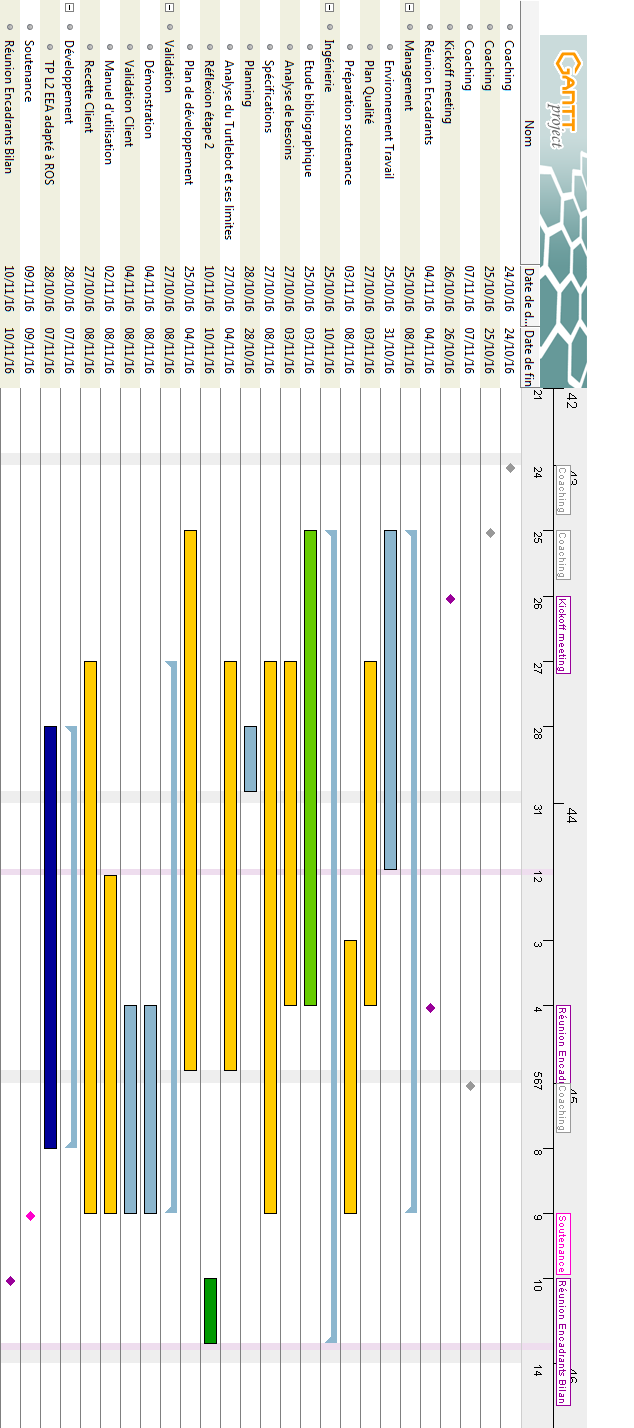
\includegraphics[width=\textwidth]{W1.png} 
  \caption{Gannt du W1}
\end{figure}

\subsection{[OK] Conclusion du projet}

Ce plan qualité vise à assurer que les dispositions prises par l’équipe pour obtenir la qualité du logiciel définie en accord avec les clients soient respectées. Avec le même objectif, le responsable qualité, soutenu par toute l’équipe, sera en charge de vérifier que les engagements pris dans le présent document auront été appliqués tout au long de l'avancement de ce projet.

Les membres de l'équipe projet sont tenus de se conformer aux dispositions décrites dans le plan d'assurance et de contrôle qualité. Le non-respect des prescriptions du Plan de Qualité constaté donne lieu à un plan d'action curatif pour corriger les effets du dysfonctionnement et éventuellement à un plan d'action préventif pour éviter que celui-ci ne se reproduise. Ce dernier plan peut entraîner une modification du plan qualité. L’utilisation de ce plan doit permettre un total succès du projet :

\begin{description}
\item [Succès du produit] : avoir un produit final qui satisfait les besoins des utilisateurs, qui a le niveau de qualité requis (tests, code propre et commenté) et qui puisse être évolutif (générique) et réutilisable (documentations)
\item [Succès de la démarche] : les demandes du client satisfaites dans les délais, les méthodes établies et le planning bien respecté
\end{description}

Le projet et les résultats obtenus seront décrits dans le bilan et exprimés lors de la présentation orale et de la démonstration publique. 

% ----------------------------

\section{Assurance qualité}

\subsection{[AFAIRE] Organisation interne}

\subsection{[AMODIFIER] Organisation externe}

La communication avec les clients se fera premièrement par courrier électronique. Les clients pourront alors répondre à toute l’équipe via l’adresse mail du groupe mise à leur disposition. Deuxièmement, des réunions hebdomadaires seront également prévues afin de tenir informés les intervenants sur l’avancement du projet. Des réunions supplémentaires pourront également être organisées si cela s’avère nécessaire. Chaque réunion sera prévue au moins 2 jours à l’avance et donnera lieu à un compte rendu de réunion. Ces comptes rendus seront envoyés par courriel, dont l’objet sera identifié VOIR PARTIE, et ils seront rédigés à partir des formulaires fournis en Annexe. Ces documents seront soumis à l’approbation dans les trois jours. De plus, toutes les informations relatives au projet, quelle que soit leur nature seront accessibles immédiatement dans nos espaces de travail VOIR PARTIE.

\subsection{[AMODIFIER] Outils}

\subsubsection{Développement}
\begin{description}
\item [Système d'exploitation : Ubuntu 14.04 LTS et ROS]
\item [Git] : Logiciel libre de gestion de versions. Nous l'utilisons pour la gestion de nos sources mais aussi pour gérer la rédaction collaborative de nos documents.
\item [Github] : Hébergeur de notre dépôt Git. L'interface Web fourni également un accès à des outils de gestion du code. Une liste d'Issues qui sera utilisé pour discuter des modifications effectuée dans les codes et un système de \textit{Pull Request} qui nous permet de valider et d'intégrer des modifications. Un wiki est également accessible via cette interface.\\ \href{https://github.com/Projet-Navigation-UPS}{[lien vers le dépôt GitHub]} 
\end{description}

\subsubsection{Documentation}
\begin{description}
\item [Unified Modeling Language (UML)] : Ce langage va nous permettre de modéliser les différents composants et le déroulement de nos programmes. La modélisation y est graphique et permet de comprendre et de communiquer simplement sur le fonctionnement d'une application complexe.
\item [Google Drive] : Système de stockage et de partage en ligne de fichiers. Il permet d'archiver et d'avoir accès aux versions finales des documents rédigés et utilisés durant le projet. \\
\href{https://drive.google.com/drive/folders/0B17hXXH2aZiVb1ZiNlhpMWk4OFE?usp=sharing}{[lien vers le dépôt Google Drive]}
\item [Cacoo] : Service en ligne de création et de partage de diagramme.
\item [LaTeX - TexMaker] : LaTeX est un langage de rédaction de document. Il permet la rédaction de document et l'intégration de plusieurs parties facilement. Nous avons décidé de choisir une distribution LaTeX commune pour s'assurer que les documents produits soient homogènes (encodage, caractères spéciaux… etc)
\end{description}

\subsubsection{Espace de travail}
\begin{description}
\item [GanttProject] : Logiciel libre de gestion de projet. Il nous permet de modéliser dans le temps l'ensemble des tâches liée au projet ainsi que leur relation entre elles.
\item [Trello] : Outil de gestion de projet en mode « Tableau de tâches ». Il nous permet d'organiser la distribution et la réalisation des tâches. Il sert également comme vecteur d'information sur la gestion du projet en général (liens des outils, documents importants… etc.).\\ \href{https://trello.com/b/eJKigNIz}{[lien vers le tableau Trello]}
\item [Placker] : Outil de gestion de projet en mode diagrammes de Gantt. Il permet de gérer les tâches d'un tableau Trello à l'aide d'un diagramme de Gantt. Il est utilisé pour surveiller l'avancement des tâches de plus bas niveau.
\item [Google Mail] : Service de messagerie électronique. Il est utilisé pour l’ensemble de nos échanges internes ou externes au projet.
\item [Google Agenda] : Service en ligne d'agenda. Utilisé pour la prise de rendez-vous et la mise en place des réunions internes et externes au groupe de projet. 
\end{description}
 
\subsection{[AMODIFIER] Standards}

\subsubsection{Gestion des documents}

Chaque document produit par le groupe projet devra comporter une page de garde reprenant les éléments nécessaires à leur suivi :
\begin{itemize}
\item Informations générales de suivi :
\begin{itemize} 
	\renewcommand{\labelitemii}{$\cdot$}
	\item Nom du document
	\item Version
	\item Date de création
	\item Date de modification
\end{itemize}
\item Auteurs du document
\item Auteur et date de la validation du document pour la version en cours.
\item Historique de révision
\end{itemize}

\noindent Processus de production des documents :
\begin{itemize}
\item Rédaction des parties du document par l'ensemble des auteurs concernés ;
\item Ajout des rédactions par \textit{commit} sur le dépôt Git. 
\item Fusion et résolution des conflits. Ajout des corrections si nécessaire ;
\item Validation finale d'une version du document. \textit{Tag} de version sur le dépôt Git ;
\item Envoi ou diffusion du document aux destinataires concernés ;
\item Archivage du document.
\end{itemize}

Il peut être nécessaire de répéter plusieurs fois la partie rédaction, ajout et fusion afin d'obtenir une version du document convenable.

\subsubsection{Objet des e-mails}

Pour des raisons de suivi, l'ensemble des e-mails est envoyé à plusieurs destinataires chacun travaillant dans des domaines différents. Pour faciliter la recherche et l'identification du contenu des e-mails, nous avons décidé de respecter la forme d'objet suivante : 

\verb|[Projet NAV - Thème] Objet du mail|

\subsubsection{Entête des fichiers}
L'entête de chaque fichier source doit être complétée afin d'expliquer leur comportement. Elle doit être mise à jour au fur et à mesure des évolutions du fichier qu'elle décrit.
Chaque entête doit permettre de comprendre facilement et rapidement les fonctionnalités codées.
Voici une liste non exhaustive des éléments à renseigner :
\begin{itemize}
\item Méthode/Fonction
\begin{itemize} 
	\renewcommand{\labelitemii}{$\cdot$}
	\item \verb|D:| Descriptif
	\item \verb|A:| Auteur(s)
	\item \verb|E:| Description des paramètres
	\item \verb|S:| Donnée(s) renvoyée(s)
	\item \verb|R:| Donnée renvoyée
	\item \verb|F:| Exceptions et/ou code(s) d'erreur(s) renvoyé(es)
\end{itemize}
\item Classe
\begin{itemize} 
	\renewcommand{\labelitemii}{$\cdot$} 
	\item Descriptif
	\item Auteur(s)
\end{itemize}
\end{itemize}

Il est recommandé de commenter au maximum le code afin de faciliter la phase de développement du projet.

\subsubsection{Nommage}

Les fichiers suivent le nommage de leur classe respective.
Pour les fichiers C++ c'est le suffixe .cpp qui sera utilisé. Pour les headers C++ le suffixe .hpp sera utilisé.
\begin{description}
\item [Classes] :
\begin{itemize}
\item Première lettre en majuscule 
\item Mélange de minuscule, majuscule. 
\item Première lettre de chaque mot en majuscule
\item Donner des noms simples et descriptifs 
\item Éviter les acronymes 
\item N’utiliser que \verb|[a-z][A-Z]| et \verb|[0-9]|
\end{itemize}

\item [Variables] : 
\begin{itemize}
\item Première lettre en minuscule
\item Mélange de minuscule, majuscule avec la première lettre de chaque mot en majuscule 
\item Donner des noms simples et descriptifs 
\item N’utiliser que \verb|[a-z][A-Z]| et \verb|[0-9]|
\end{itemize}


\item [Constantes] :
\begin{itemize}
\item Tout en majuscule 
\item Séparer les mots par des underscore
\item Donner des noms simples et descriptifs 
\item N’utiliser que \verb|[A-Z]| et \verb|[0-9] |
\end{itemize}

\end{description}

\subsubsection{Découpage du code}

Il est important que le code soit suffisamment découpé. La taille des fichiers ne devrait pas excéder 1000 lignes et chaque fonction (ou méthode) ne devrait pas dépasser la centaine de lignes au grand maximum. Les headers et les fichiers source séparent les déclaration des définitions.

L'indentation doit être strictement respectée et doit correspondre à un espacement de 4 caractères. La taille des lignes ne doit pas dépasser 80 caractères.


\subsubsection{Workflow}

Voici une description du \textit{workflow} utilisé pour réaliser les tâches de développement de notre projet :
\begin{itemize}
\item La branche \textit{master} contient uniquement un système complet en état de fonctionner. Elle est protégée en écriture par le Scrum Master.
\item La branche \textit{develop} est notre branche de travail par défaut.
\item Pour travailler sur une nouveauté, on travaille directement sur la branche \textit{develop} ou on créé une nouvelle branche à partir de la branche \textit{develop} lorsque la fonctionnalité développée demande au moins un jour de travail.
\item Lorsque la branche de travail est prête, on ouvre une \textit{Pull Request} pour demander une intégration à la branche master au Scrum Master.
\item Validation et/ou corrections des modifications. Une fois que cela est fait on fusionne dans la branche \textit{master}.
\item Déploiement du code de la branche \textit{master} sur le système.
\end{itemize}

Il est également important d'alimenter le \textit{wiki} lorsqu'un membre du groupe estime qu'une information importante concernant les développements doit être partagée aux utilisateurs et/ou aux membres du projet. La forme de rédaction est libre mais chaque page doit être référencée avec un titre précis et explicite sur le contenu qu'elle présente.

Il est conseillé de respecter le format suivant pour les préfixes des \textit{commit} sur le dépôt Git :
\begin{itemize}

\item \verb|ADD| : Ajout de fichiers, de méthodes, d'une configuration, d'un texte \ldots etc...
\item \verb|ENH| : Amélioration d'un élément déjà présent
\item \verb|RM| : Suppression d'un fichier, d'une méthode, d'une classe, d'un texte \ldots etc...
\item \verb|BUG| : Correction d'un bug.
\item \verb|TEST| : Relatif aux tests.
\item \verb|DOC| : Relatif à la documentation.
\end{itemize}

Il est nécessaire que l'ensemble des membres du projet utilisent la liste d'\textit{Issues} pour pouvoir effectuer et archiver les différents discussions sur le code du projet. Il est possible d'ouvrir et de fermer ces \textit{issues}. Lorsqu'un \textit{commit} est en rapport avec une \textit{issue} il doit être relié avec celui-ci (i.e. \verb|BUG : add method close #12| ce commit ferme automatiquement l'\textit{issue} numéro 12).


\section{[OK] Analyse des risques}
\begin{figure}
  \centering
\noindent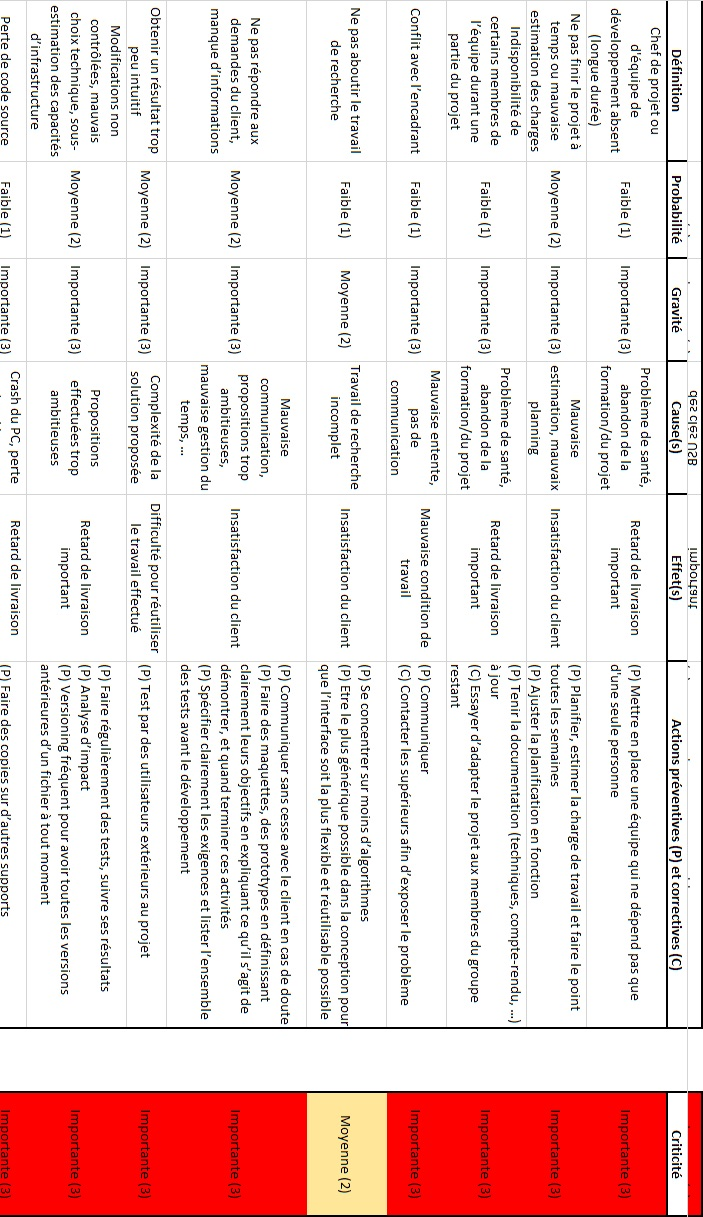
\includegraphics[width=\textwidth]{risques.jpg} 
  \caption{Analyse de risques}
\end{figure}

\section{[AFAIRE] Validation}


\newpage
\listoffigures
\newpage

\section*{ANNEXE}
\subsection*{Template de compte-rendu de réunion}

\noindent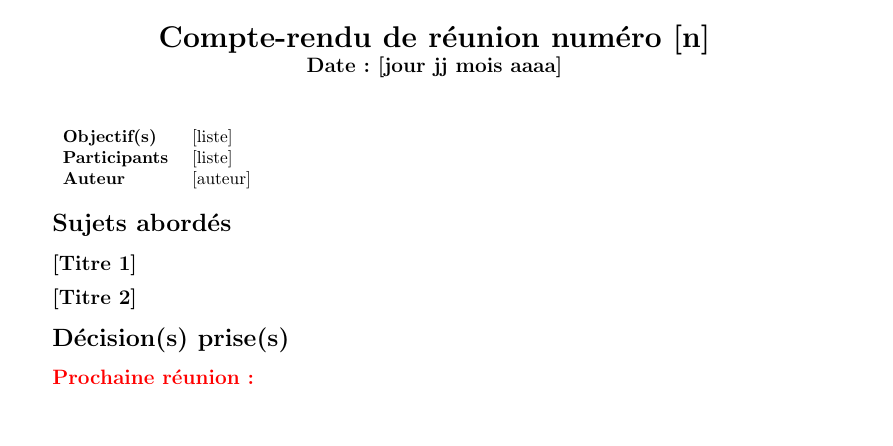
\includegraphics[width=\textwidth]{tmp-cr.png} 

\end{appendix}

\end{document}

